\documentclass[letterpaper]{article}
\usepackage{adjustbox}

\usepackage{aaai}
\usepackage{times}
\usepackage{helvet}
\usepackage{courier}
\setlength{\pdfpagewidth}{8.5in}
\setlength{\pdfpageheight}{11in}

\usepackage{amsmath}
\usepackage{color}
\usepackage{url}
\usepackage{graphicx}

\RequirePackage{etex}
\RequirePackage{amsmath}
\RequirePackage{amsthm}
\RequirePackage{amsbsy}
\RequirePackage{amsfonts}
\RequirePackage{array}
\RequirePackage{aliascnt}

\newcommand{\comment}[1]{}
\newtheorem{theorem}{Theorem}
\newtheorem{lemma}{Lemma}
\newtheorem{definition}{Definition}
\newtheorem{corollary}{Corollary}

\newcommand{\tuple}[1]{\ensuremath{\left \langle  #1 \right \rangle }}
\newcommand{\commentout}[1]{}
\newcommand{\set}[1]{\{#1\}}

\theoremstyle{definition}
\newtheorem{example}{Example}

\title{Qualitative Planning under Partial Observability in Multi-Agent Domains}

\author{
Ronen I. Brafman \\
Ben-Gurion University \\
Beer-Sheva 84105, Israel\\
brafman@cs.bgu.ac.il
\And Guy Shani\\
Ben-Gurion University \\
Beer-Sheva 84105, Israel\\
shanigu@cs.bgu.ac.il
\And
Shlomo Zilberstein\\
University of Massachusetts\\
Amherst, MA 01003, USA\\
shlomo@cs.umass.edu}


\begin{document}

\maketitle

\begin{abstract}
Decentralized POMDPs (Dec-POMDPs) provide a rich, attractive model for planning under uncertainty and partial observability in cooperative multi-agent domains with a growing body of research. In this paper we formulate a qualitative, propositional model for multi-agent planning under uncertainty with partial observability, which we call Qualitative Dec-POMDP (QDec-POMDP). We show that the worst-case complexity of planning in QDec-POMDPs is similar to that of Dec-POMDPs. Still, because the model is more ``classical'' in nature, it is more compact and easier to specify.  Furthermore, it eases the adaptation of methods used in classical and contingent planning to solve problems %% to which Dec-POMDPs solution techniques cannot scale up.
that challenge current Dec-POMDPs solvers.
In particular, in this paper we describe a method based on compilation to classical planning, which handles multi-agent planning problems significantly larger than those handled by current Dec-POMDP algorithms.
\end{abstract}

\section{Introduction}
Many problems of practical importance call for the use of multiple autonomous agents that work together to achieve a common goal.
For example, disaster response teams typically consist of multiple agents that have multiple tasks to perform,
some of which
require or can benefit from the cooperation of multiple agents. In such domains, agents typically have partial information, as they can sense their immediate surroundings only.
And because agents are often located in different positions and may even have different sensing abilities, their runtime information states differ.  Sometimes, this can be overcome using communication, but communication infrastructure can be damaged, and even if it exists,
communication may be costly (in terms of time and resources) and should be reasoned about explicitly.

Decentralized POMDPs (Dec-POMDPs) offer a rich model for capturing such multi-agent planning problem~\cite{Bernstein02,Seuken08}. Dec-POMDPs extend the single agent POMDP model to account for multiple agents with possibly different information states, but the complexity of the Dec-POMDP model has limited its applicability.  In this paper we define and study a conceptually simpler model for multi-agent planning that extends the single-agent contingent planning model.  We call this new model \emph{Qualitative Dec-POMDP} (QDec-POMDP).


In terms of worst-case complexity, we show that QDec-POMDPs are no easier than Dec-POMDPs. %% So what is their advantage?
Nevertheless, a multi-agent contingent planning formalism offers two main advantages. First, being geared to propositional (a.k.a.~factored) state models, it allows for more convenient model specification, as opposed to flat state models that characterize much of the work on Dec-POMDPs.  Second, much like contingent planning, it is more amenable to the use of current classical planning methods, which are quite powerful.
Thus, it could allow us to solve much larger problems. Indeed, one of our main contributions is a compilation method from QDec-POMDPs to classical planning, allowing us to tackle domains larger than those that can be solved by current Dec-POMDP algorithms.

Of course, the qualitative contingent planning model is less expressive in that it specifies the possible outcome states without their likelihood.  But this is an advantage in cases where it is difficult to specify a richer, quantitative model, or when such models are too complex to solve.  Furthermore, a solution to a qualitative model can provide guidance and heuristics for methods that operate on the quantitative model.  Alternatively, one could use information from the quantitative model to bias choices made by a qualitative counterpart, e.g., when state sampling techniques are used, thus gradually moving from qualitative to quantitative.

In the next section we introduce the formal QDec-POMDP model.  We start with an analysis of the complexity of solving a flat state-space qualitative model.  This makes clear the impact of the move from a quantitative Dec-POMDP model, for which
complexity results exist in that form. Next, we take a closer look at the issue of belief state representation, which is much more complex than in the single agent case. Here we still consider a flat state space model for semantic clarity.  Next, we introduce a factored model, in the spirit of contingent planning models. Focusing on a deterministic variant of this model, we suggest an offline compilation method for its solution, and describe its empirical performance. The earlier discussion of belief states will help us understand an essential simplification made by this model.  We end by discussing some of the challenges faced in designing an online algorithm.



\section{Model Definition}
We start with the basic definition of a flat-space QDec-POMDP.
\begin{definition} A qualitative decentralized partially observable Markov decision process
(QDec-POMDP) is a tuple ${\cal Q} = \langle  I, S, b_0,\{A_i\}, \delta, \{\Omega_i\}, O, G, T\rangle$
where
\begin{itemize}
\setlength{\itemsep}{-1pt}
\item $I$ is a finite set of agents indexed $1,...,m$.

\item $S$ is a finite set of states.

\item$b_0 \subset S$ is the set of states initially possible.

\item $A_i$ is a finite set of actions available to agent $i$ and
$\vec{A} = \otimes_{i \in I} A_i$ is the set of joint actions, where
$\vec{a} = \tuple{a_1,...,a_m}$ denotes a particular joint action.

\item $\delta: S \times \vec{A} \rightarrow 2^S$ is a non-deterministic Markovian transition function. $\delta(s, \vec{a})
$ denotes the set of possible outcome states after taking joint action $\vec{a}$ in state $s$.

\item $\Omega_i$ is a finite set of observations available to agent $i$ and
$\vec{\Omega} = \otimes_{i \in I} \Omega_i$ is the set of joint
observation, where $\vec{o} = \tuple{o_1,...,o_m}$ denotes a particular joint
observation.

\item $\omega : \vec{A} \times S \rightarrow 2^{\vec{\Omega}}$ is a {\em non-deterministic\/} observation function. $\omega(\vec{a}, s)$
denotes the set of possible joint observations $\vec{o}$ given that
joint action $\vec{a}$ was taken and led to outcome state $s$. Here $s \in S,\, \vec{a}
\in \vec{A},\, \vec{o} \in \vec{\Omega}$.

\item $G \subset S$ is a set of goal states.

\item $T$ is a positive integer representing the horizon.

\end{itemize}
\label{11_def:DEC-POMDP}
\end{definition}
Our model allows for non-deterministic action effects as well as non-deterministic observations. That is, we allow a set of possible global states to result from a single joint action, and we also allow multiple possible observations per outcome state.
Additionally, our model assumes a shared initial belief state, as most Dec-POMDP models. The case where agents have different initial belief states is very important, as it corresponds to the situation in on-line planning, but is also very challenging.

We represent the local plan of each agent using a \emph{policy tree} $q$, which is a tree with branching factor $|\Omega|$ and depth $T$.  Each node of the tree is labeled with an action and each branch is labeled with an observation.  To execute the plan, each agent performs the action at the root of the tree and then uses the subtree labeled with the observation it obtains for future action selection.
If $q_i$ is a policy tree for agent $i$ and $o_i$ is a possible observation for agent $i$, then $q_{i_{o_i}}$ denotes the subtree that corresponds to the branch labeled by $o_i$.

Let $\vec{q} = \langle  q_1, q_2, \cdots, q_m \rangle$ be a vector of policy trees.  $\vec{q}$ is also called a {\em joint policy}.
We denote the joint action at the root of $\vec{q}$ by $\vec{a}_{\vec{q}}$, and for an observation vector
$\vec{o}=o_1,\ldots, o_m$, we define $\vec{q}_{\vec{o}}= \langle  q_{1_{o_1}},\ldots q_{m_{o_m}}\rangle$.

We later suggest algorithms to compute a joint policy that solves a given QDec-POMDP (guarantee goal reachability).

\section{Complexity of QDec-POMDP}

We now analyze the complexity of generating plans in our proposed model, compared with policy generation in the traditional Dec-POMDP model.

We first characterize the set of states reachable via a joint policy $\vec{q}$. Intuitively, if all states reached by time $T$ are goal states,
the joint policy is a solution to the QDec-POMDP.  To do so, we define the set of pairs of the form (global state, joint policy) that are reachable, denoted by $\beta$.
The base case, $\beta_0$, corresponds to initially possible states and the full depth-$T$ joint policy $\vec{q}$: $\beta_0 = \{(s,\vec{q}) | s \in b_0\}$.  We define $\beta_{t}$ inductively:
\begin{equation} \nonumber
\beta_{t} = \{ (s', \vec{q}_{\vec{o}}) ~|~
(s,\vec{q}) \in \beta_{t-1}, ~s' \in \delta(s,\vec{a}_{\vec{q}}), ~\vec{o} \in \omega(\vec{a},s') \}
\label{eq:bu}
\end{equation}



We can now formally define a solution to a QDec-POMDP using our $\beta$ notation:
\begin{definition}
A given depth-$T$ joint policy $\vec{q}$ is a solution to a QDec-POMDP {\cal Q} ~iff~
$\forall s : (s,\emptyset) \in \beta_T ~\Rightarrow~ s \in G$.
\end{definition}
\noindent Note that at time $T$ the remaining policy trees are empty.

\begin{definition}
Let QDec-POMDP$_m$ denote the problem of finding a joint policy $\vec{q}$ that is a solution of a given $m$-agent
QDec-POMDP ${\cal Q} = \langle  I, S, \{A_i\}, \delta, \{\Omega_i\}, O, G, T\rangle$ (i.e., $|I|=m$).
\end{definition}

We now analyze the complexity of finding such solutions.
\begin{theorem}
For all $m\geq2$, if $|T|\leq S$, then \\ QDec-POMDP$_m \in$ NEXP.
\end{theorem}

\begin{proof}
We show that a nondeterministic machine can solve an instance of QDec-POMDP$_m$ using at most exponential time.  To start, we guess a joint policy $\vec{q}$.
A joint policy includes $m$ policy trees, each of size $O(|\Omega|^T)$.  Overall, the size is $O(m|\Omega|^T)$, and because $T< |S|$, the joint policy can be generated in exponential time.  Given a joint policy, the update of the belief state $\beta_t$ can be performed in exponential time: $\beta_{t}$ can be larger than $\beta_{t-1}$ by at most a multiplicative factor of $|S|$, and the update takes polynomial time in the size of $\beta_{t}$. Thus repeating this process $T$ times may require at most exponential time.
Finally, all we need is to verify that $ \forall s :~ (s,\emptyset) \in \beta_T ~\Rightarrow~ s \in G $.
\end{proof}

\begin{theorem}
For $m\geq2$, QDec-POMDP$_m$ is NEXP-Hard.
\end{theorem}

\begin{proof}
The proof is similar to the one presented by~\cite{Bernstein02} for Dec-POMDPs.  It follows a reduction of the TILING problem~\cite{Lewis78,Papadimitriou94}, which is NEXP-complete, to the QDec-POMDP$_2$ problem.  We only sketch the argument here.

TILING involves a given board size $n$ (represented in binary), a set of tile types $L \!=\! \{tile_0, ..., tile_k\}$,
and a set of binary horizontal and vertical compatibility relations $H, V \!\in\! L \!\times\! L$.

A tiling $f$ is \emph{consistent} \emph{iff}
(a) $f(0,0) = tile_0$, and (b) for all $x,y$ $\langle  f(x,y), f(x+1,y) \rangle \in H$ and
$\langle  f(x,y), f(x,y+1) \rangle \in V$.  That is, adjacent tiles satisfy the compatibility relations.
The decision problem is to determine, given $n, L, H, V$, whether a consistent tiling exists.

The basic idea is to create a two-agent QDec-POMDP that randomly selects two tiling locations bit by bit, informing one agent of the first location and the other agent of the second location. The agents' local policies are observation-history based, so the agents can base their future actions on the tiling locations given to them.  After generating the locations, the agents are simultaneously queried to place tiles at some locations. The QDec-POMDP problem is designed such that the agents reach the goal \emph{iff} their answers to the query are based on some agreed upon solution of the tiling problem.  Here is a brief discussion of the phases of the original proof from~\cite{Bernstein02} and the relevant changes needed for the QDec-POMDP model.

\begin{description}
\setlength{\itemsep}{0pt}
\item [Select Phase]  Using nondeterminism, the system generates two random bit positions and values.  They are memorized as part of the state and not observed by the agents.

\item [Generate Phase] Using nondeterminism, the system generates two tile locations and reveals one to each agent via their observation streams.

\item [Query Phase] Each agent is queried for a tile type to place in the location specified to it.

\item [Echo Phase] The agents are now required to echo their tile locations.  Only one position (not known to the agents) is verified by the system per observation stream.  Making an error in the echo phase leads to a dead-end, from which the goal cannot be reached.  During the echo phase, the system tracks the adjacency relationship between the tile locations.

\item [Test Phase]  The system checks whether
the tile types provided in the query phase come from a single consistent tiling. If the tile types violate any of the constraints, a dead-end state is reached.  Otherwise, the goal is reached.

\end{description}
Similar to the original proof, if there exists a consistent tiling, then there must exist a joint policy for the constructed QDec-POMDP$_2$ that reaches the goal state. Likewise, there is no way to \emph{guarantee} goal reachability without the agents being faithful to a single consistent tiling.
\end{proof}

Note that the QDec-POMDP constructed for the proof is in fact a QDec-MDP (i.e., the observations of the two agents combined provide full information on the state of the system).  Therefore, QDec-MDP$_2$ is NEXP-Hard as well.

\begin{corollary}
For all $m\geq2$, both QDec-POMDP$_m$ and QDEC-MDP$_m$ are NEXP-complete.
\end{corollary}

It is somewhat surprising that the qualitative model with its different objective (goal reachability versus maximizing expected reward) has the same complexity as the standard Dec-POMDP model. In some sense, this confirms the intuition that the main source of complexity is decentralized operation with partial information, not stochastic actions.

\section{Belief States and Joint Policies}
The notion of the agent's belief state plays a central role in algorithms for solving problems with partial observability and in the representation and computation of policies. In this section, we seek to understand belief states in QDec-POMDPs, explain some simplification we %% later
make, and use this to provide an alternative representation for a joint policy.


\subsection{Online Local Belief States}
We begin with a definition of a local belief state of an agent in the context of a known joint-policy tree. This definition is useful for reasoning about the information state of an agent online.  However, it is not useful for the generation of a joint-policy, as it assumes a fixed policy.

Each agent can maintain a belief state $\beta_i^t$ at time $t$ that reflects its own experience.  The belief state includes all the possible pairs of the form {\em system state} and {\em joint policy}. Agent $i$ knows its own policy tree, so all joint policies considered possible in its belief state must agree with its own, actual, policy tree.

The initial belief state of agent $i$ is $\beta_i^0 = \{(s_0, \vec{q}) | s_0 \in b_0\}$ where $\vec{q}$ is the initial vector of policy trees for all the agents.  Let  $a_i^t$ be the action agent $i$ executes at time $t$, and $o_i^t$ the observation it obtains.
We define $\beta^{t}$ inductively as follows:
\begin{eqnarray}
\scriptsize
\beta_i^{t}  & = & \{ ( s_t, \vec{q}_{\vec{o}} ) ~|~ (s_{t-1},\vec{q}) \in \beta_i^{t-1}, \\ \nonumber
& & \hspace{46pt} s_t \in \delta(s_{t-1}, \vec{a}_{\vec{q}}), \\ \nonumber
& & \hspace{46pt} \vec{o} \in \omega(\vec{a}_{\vec{q}},s_t), ~\vec{o}[i] = o^t_i \}
\end{eqnarray}
The only difference between the global update of $\beta^t$ and the local update is the added condition $\vec{o}[i] = o^t_i$, which means that we only include outcome states $s_t$ that produce the actual observation that agent $i$ obtained.  That is, we use the local information of agent $i$ to filter states that are inconsistent with its knowledge.

This belief state update scheme is valid when the joint policy is fixed in advance in the form of policy trees.  But if we want to have policies that depend on these local belief states we run into a problem.  The actions of the other agents depend on their beliefs that in turn depend on their actions. Without resolving this circularity, it is hard to generate plans conditioned on local beliefs.


\subsection{Offline, Policy Independent Belief States}
Most existing methods for planning under partial observability rely on a ``nice-to-manage'', policy-independent notion of belief state.
These methods include, for example, search in belief state space, the computation of a real-valued function over belief states, as in POMDPs, and the generation of a policy that maps belief states to actions.

In the multi-agent case there is no longer a single belief state, but we can replace that with the notion of a history. A \emph{history} is a sequence of
states and actions, of the form $(s_0,a_1,s_1,\ldots,a_n,s_n)$, denoting the initial state, the initial action, the resulting state, etc.
If $h=(s_0,a_1,s_1,\ldots,a_n,s_n)$, let $h_s(k)= s_k$ and $h_a(k)=a_k$.
Initially, every agent's belief state is $\beta_i^0 = \{(s_0) | s_0 \in b_0\}.$
We define $\beta^t_{\beta^{t-1},a_i,o_i}$, the new belief state of agent $i$ at time $t$ after executing $a_i$ and observing $o_i$ in belief state $\beta^{t-1}$, as follows: \\[-12pt]

\begin{eqnarray}
\scriptsize
\beta^t_{\beta^{t-1},a_i,o_i} & = & \{ (h\; \circ (\vec{a}_t,s_{t})) ~|~ h\in\beta^{t-1}, \\  \nonumber
&&~s_{t}\in\delta(h_s(t-1), \vec{a}_t),~\vec{a}_t[i] = a_i,\\  \nonumber
&& ~\vec{o} \in \omega(\vec{a}_t,s_{t}), ~\vec{o}[i] = o_i\}
\end{eqnarray}



That is, those histories that extend current histories with a joint action that is consistent with the local action executed by the agent, and
with a state which is the result of applying that joint action to the last state of the history, such that this last state and action can induce a
joint-observation consistent with an agent's local observation.

In the (qualitative) single agent case, due to the Markovian assumption, one can simply maintain the set of last states of the above histories, rather than the entire history, i.e., maintaining the set of currently possible states. Unfortunately, to the best of our knowledge, such a ``truncation'' is not possible in the multi-agent case without sacrificing completeness.
The reason is that different histories that led one agent to the same state, lead to different states of information for other agents. Thus, the set of last states in histories considered possible by an agent only approximates its state of knowledge.  We will employ this approximation in the planning algorithm introduced later, referring to it as {\em set-of-possible-states\/} approximation.

Initially, every agent's belief state is $\beta_i^0 = \{(s_0) | s_0 \in b_0\}$.  The estimated set of possible states for agent $i$ at time $t$ given the estimated belief state at time $t-1$, action $a_i$ by the agent, and observation $o_i$
is defined as follows: \\[-12pt]

\begin{eqnarray}
\scriptsize
\beta^t_{\beta^{t-1},a_i,o_i} &=& \{ s_{t}~: ~s_{t-1}\in\beta^{t-1},\\ \nonumber
&& s_{t}\in\delta(s_{t-1},\vec{a}_t), \vec{a}_t[i] = a_i,\\ \nonumber
&&\vec{o} \in \omega(\vec{a}_t,s_{t}), ~\vec{o}[i] = o_i\}
\end{eqnarray}

\subsection{Global Policy Tree}
To describe a joint policy, we used a vector $\vec{q}$ of individual policy trees. An alternative description is a global policy tree,
which we denote by $q_g$. Its definition is identical to that of an individual policy tree, except that nodes are labeled by {\em joint} actions, and edges are labeled by {\em joint} observations.

Unfortunately, some general policy trees do not correspond to any joint policy. If two nodes in the global policy tree correspond to branches
that would yield the same history for agent $i$, i.e., agent $i$ cannot distinguish between these branches, the action assigned to $i$ in these
nodes must be identical.

Thus, let $q_g$ be a policy tree, and let $b_0$ be the initial belief state. For every node $n$, let $\vec{b}(n)= b_1(n),\ldots,b_m(n)$ be the
vector of agents' belief states given the history that corresponds to the path to this node. $q_g$ is {\em executable} if for every agent $i=1,\ldots, m$ and every two nodes $n,n'$ in $g_p$, if $b_i(n)=b_i(n')$ then the $i^{th}$ component of the joint actions associated with $n$ and $n'$ must be identical.

Although joint policies are easier to execute -- they contain an explicit policy for each agent -- global policy trees are a better fit for
the compilation approach that we describe below, because they are closer in form to (single-agent) classical plans over joint actions:
Instead of generating joint policy trees consisting of $m$ local policies, our translation method will seek a single {\em executable\/} global policy tree. To ensure that the global tree is executable, we will enforce the constraint described above
while using the set-of-possible-states approximation for agents' state of knowledge.
Because this approximation is sound, i.e., two histories that the agent cannot distinguish with will always
yield two identical sets of possible states (but not vice versa), we are guaranteed that the global policy tree is indeed executable.

\section{Factored Representation of QDec-POMDP}

A factored representation of a planning problem %% can allow for compact representations of problems, as well as
makes it more compact and facilitates development of
efficient algorithms that leverage the factored structure. With a few exceptions~\cite{Oliehoek08,KZTijcai11}, little work has focused on exploiting such factored models for Dec-POMDPs.  Moreover, existing factored Dec-POMDPs
use a ``flat'' state representation {\em per} agent (one state variable per agent) as opposed to multiple generic state variables that describe compactly the entire state space.

In this section we describe a factored specification of a QDec-POMDP model, motivated by the classical STRIPS and PDDL languages. We propose a PDDL-like representation that is much more compact than the SPUDD-like representation used in some factored Dec-POMDPs.
At present, our language does not support non-deterministic observations. Although conceptually simple and easy to define in multi-valued settings, formalizing non-deterministic observations in the boolean STRIPS setting is not straightforward, and is thus left for future work. In what follows we slightly abuse notation by overloading previously defined terms.

\begin{definition}
A factored QDec-POMDP  is a tuple $\langle I,P,\vec{A},\mathit{Pre},\mathit{Eff},\mathit{Obs},b_0,G\rangle$ where $I$ is a set of agents, $P$ is a set of propositions, $\vec{A}$ is a vector of individual action sets,  $\mathit{Pre}$ is the precondition function,
$\mathit{Eff}$ is the effects function, $b_0$ is the set of initially possible states, and $G$ is a set (conjunction) of goal propositions.
The state space $S$ consists of all truth assignments to $P$, and each state can be viewed as a set of literals.
\end{definition}

The precondition function $\mathit{Pre}$ maps each individual action $a_i\in A_i$ to its set of preconditions, i.e., a set of literals that must
hold whenever agent $i$ executes $a_i$. Preconditions are local, i.e., defined over $a_i$ rather than $\vec{a}$, because each agent must ensure that the relevant preconditions hold prior to executing its part of the joint action. We extend $\mathit{Pre}$ to be defined over joint actions $\{\vec{a}=\langle a_1,..,a_m\rangle : a_i \in A_i\}$ (where $m=|I|$):
$\mathit{Pre}(\langle a_1,..,a_m\rangle) = \cup_i \mathit{Pre}(a_i)$.

The effects function $\mathit{Eff}$ maps joint actions into a set of pairs $(c,e)$ of conditional effects, where $c$ is a conjunction of literals and $e$ is a single literal, such that if $c$ holds before the execution of the action $e$ holds after its execution. Thus, effects are a function of the {\em joint\/} action rather than of the local actions, as can be expected, due to possible interactions between local actions. For the sake of semantic clarity, we assume that if $(c,e)$ and $(c',e')$ are conditional effects of the same joint action, then $c$ and $c'$ are inconsistent.
Here we focus on deterministic effects, but one can model non-deterministic effects simply by allowing for multiple pairs of the form
$(c,e),(c,e')$ representing alternative outcomes of the action under the same conditions.

The preconditions and effects functions together define the transition function between states given actions.

For every joint action $\vec{a}$ and agent $i$, $\mathit{Obs}(\vec{a},i)=\{p_1,\ldots,p_k\}$, where $p_1,...,p_k$ are the propositions
whose value agent $i$ observes after the joint execution of $\vec{a}$. The observation is private -- i.e., each agent may observe
different aspects of the world, and we assume that the observed value is correct and corresponds to the post-action value of
these variables.


A solution to the factored model is identical to that used for the flat model. We can use joint policy trees or executable global policy trees, as
discussed earlier.


\begin{figure}[t]
\centering
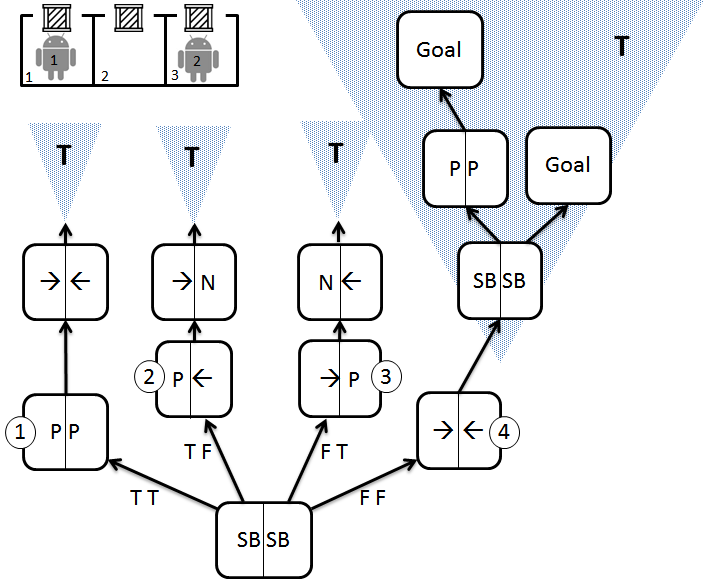
\includegraphics[width=3.5in]{JointPolicyTree.png}
\label{fig:JointPolicyTree}
\caption{\small{Illustration of Example\;1 showing the box pushing domain with 2 agents and a possible joint policy tree with nodes labeled by joint actions. Possible agent actions are sensing a box at the current agent location (denoted $SB$), moving (denoted by arrows), pushing a box up (denoted $P$), and no-op (denoted $N$).  On the second level of the tree, nodes marked 1 and 2 must have the same action for agent 1 (push up in this case), because agent 1 cannot distinguish between these two nodes. Likewise for nodes 2 and 4 with respect to agent 2 that cannot distinguish between them.}}
\end{figure}

\begin{example}
\label{ex:BoxPushing}
We now illustrate the factored QDec-POMDP model using a simple box pushing domain (Figure 1).%~\ref{fig:JointPolicyTree}).
In this example there is a one dimensional grid of size 3, with cells marked 1-3, and two agents, starting in cells 1 and 3. In each cell there may be a box, which needs to be pushed upwards. The left and right boxes are light, and a single agent may push them alone. The middle box is heavy, and requires that the two agents push it together.

We can hence define $I=\{1,2\}$ and $P=\{\mathit{AgentAt}_{i,pos},\mathit{BoxAt}_{j,pos}\}$ where $pos \in \{1,2,3\}$ is a possible position in the grid, $i \in \{1,2\}$ is the agent index, and $j \in \{1,2,3\}$ is a box index. In the initial state each box may or may not be in its corresponding cell --- $b_0=\mathit{AgentAt}_{1,1} \wedge \mathit{AgentAt}_{2,3} \wedge (BoxAt_{j,j} \vee \neg BoxAt_{j,j})$ for $j=1,2,3$. There are therefore 8 possible initial states.

The allowed actions for the agents are to move left and right, and to push a give box up. There are no preconditions for moving left and right, i.e. $\mathit{Pre(Left)}=\mathit{Pre(Right)}=\phi$. To push up box $j$, agent $i$ must be in the same place as the box. That is, $\mathit{Pre(PushUp_{i,j})}=\{\mathit{AgentAt}_{i,j},\mathit{BoxAt}_{j,j}\}$. The moving actions transition the agent from one position to the other, and are independent of the effects of other agent actions, e.g., $\mathit{Right}_{i}=\{(\mathit{AgentAt}_{i,1},\neg \mathit{AgentAt}_{i,1} \wedge \mathit{AgentAt}_{i,2}),(\mathit{AgentAt}_{i,2},\neg \mathit{AgentAt}_{i,2} \wedge \mathit{AgentAt}_{i,3})\}$. The only truly joint effect is for the actions that contain a component $\mathit{PushUp}_{i,2}$, where box 2 is the heavy box --- $\mathit{Eff}(\mathit{PushUp}_{1,2},a_2)$ where $a_2$ is some other action, are identical to the independent effects of action $a_2$, while $\mathit{Eff}(\mathit{PushUp}_{1,2},\mathit{PushUp}_{2,2})=\{(\phi,\neg BoxAt_{2,2})\}$, that is, if and only if the two agents push the heavy box jointly, it (unconditionally) gets moved out of the grid.

We define sensing actions for boxes --- $\mathit{SenseBox_{i,j}}$, with precondition $\mathit{Pre(SenseBox_{i,j})}=AgentAt_{i,j}$, no effects, and $\mathit{Obs(SenseBox_{i,j})}=BoxAt_{j,j}$.
The goal is to move all boxes out of the grid, i.e., $\bigwedge_j \neg BoxAt_{j,j}$.

\end{example}



\begin{table*}[t]
\centering
\caption{\small{Execution time (seconds) for different box pushing domains, comparing our translation-based QDec-POMDP approach, and two Dec-POMDP solvers, IPG and GMAA-ICE with the $Q_{MDP}$ heuristic.
A model is defined by its width (W), length (L), and number of boxes (B). Average depth denotes the average depth of leaves in the policy tree. Expected cost was reported by the GMAA-ICE solver.
}}
\small
\begin{tabular}{|c|c|c||c|c|c|c|c|}
\hline
Domain & $|S|$ & $|b_0|$ & QDec- & Avg & IPG & GMAA- & Expected \\
$W,L,B$ &  &  & POMDP & depth & IPG & ICE & cost \\
\hline
2 , 2 , 2 & 256 & 4 & 12.79 & 2 & 450 & 15.32 & 2 \\
2 , 3 , 2 & 1296 & 4 & 25.39 & 2 & $\times$ & 59.67 & 2  \\
2 , 3 , 3 & 7776 & 8 & 48.42 & 5 & $\times$ & 732.59 & 5 \\
3 , 3 , 3 & 59049 & 8 & 66.47 & 6 & $\times$ & $\times$ & $\times$ \\
\hline
\end{tabular}
\label{tbl:Results}
\end{table*}




\section{Compilation-Based Method}

We now present a method for solving QDec-POMDP problems using a compilation approach to classical planning. Our approach generates a planning problem whose solution corresponds to an executable global plan tree, branching on agent observations. It relies on the approximate, sound, but incomplete notion of belief state, as discussed earlier.

The compilation method is currently designed for deterministic QDec-POMDPs, i.e., ones where actions have deterministic effects. The method could in principal be expanded to handle non-determinism by embedding the uncertainty of action effects into the uncertainty of the initial belief \cite{Yoon}, but this will clearly impact the solution time and size.  We hence leave discussion of efficient handling of non-deterministic effects to future research.

A classical planning problem is a tuple $\pi=\langle P,A,s_0,G\rangle$ where $P$ is a set of propositions, $A$ is a set of actions, $s_0$ is the initial state, and $G$ is a set of goal propositions. We use a translation method inspired by the MPSR translation method \cite{MPSR} and improves upon it. An important concept in this translation is {\em distinguishability} between states. We say that we can distinguish at runtime between two states $s,s'$, denoted $\neg s/s'$, if we observed the value of some proposition $p$ which is true in $s$ and false in $s'$. In our translation we have two types of distinguishability --- when a single agent can distinguish between states based on its own observations, denoted $\neg s/s'|i$, and when the combined observations of the agents can distinguish between states, denoted $\neg s/s'$, as in MPSR.

Given a factored QDec-POMDP problem $\pi=\langle  I,P,\vec{A}=\{A_i\},\mathit{Pre},\mathit{Eff},\mathit{Obs},b_0,G\rangle$ defined as in the previous section we create the following classical planning problem $\pi_c=\langle P_c,A_c,s_{0_c},G_c\rangle$:

{\bf Propositions} $P_c = \set{p/s : p\in P , s\in S}\cup\set{\neg s/s' : s,s'\in S}\cup\set{\neg s/s'|i : s,s'\in S, i \in I}.$
Propositions of the form $p/s$ capture the value at run time of $p$ when $s$ is the true initial state.
Propositions of the form $\neg s'/s|i$ denote that at run-time, if $s$ is the true
initial state, then agent $i$ has gathered sufficient data to conclude that $s'$ cannot be the true initial state, i.e., to distinguish between state $s$ and $s'$. These propositions allow us to define the agent-specific belief state during execution, and will be used later to enforce the constraint on actions at the same level explained in the previous section.
Propositions of the form $\neg s'/s$ allow us to distinguish between states that at least one of the agents can distinguish between. These propositions allow us to define the joint belief state during plan construction.

{\bf Actions} For every joint action $\vec{a}$ and every subset of $S'\subseteq b_0$, $A_c$ contains an action $a_{S'}$. This action
denotes the execution of $\vec{a}$ when the set of possible states is $S'$ ($a_{S'}$ has no effect on states outside $S'$). It is defined as follows:\\
\emph{pre}($\vec{a}_{S'}$) =  $\{p/s : s \in S', p\in \mbox{\emph{pre}}(\vec{a})\} \cup\{\neg s'/s : s' \in S', s \in b_0\setminus S'\}$. That is, the preconditions must hold prior to applying the action in all states for which this action applies, {\em and} the joint knowledge of the agents must be sufficient to distinguish between any state in $S'$ and every state {\em not} in $S'$. Thus, the plan can choose action $a_{S'}$ only when the current belief state is $S'$, and all action preconditions are known to hold in $S'$.

For every $(c,e)\in $ \emph{effects}($a$), \emph{effects}($a_{S'}$) contains the following conditional effects:
\begin{itemize}
\setlength{\itemsep}{-1pt}
\item For each $s \in S'$, $(c/s,e/s)$ --- the effect applied to every state in $S'$.
\item $\set{(p/s \wedge \neg p/s' , \neg s/s'|i)}$ --- for every $p$ observable by agent $i$, and every two states $s,s'\in S'$, if the states disagree on $p$, then agent $i$ can distinguish between the states following the observation of the value of $p$.
\end{itemize}



{\bf Initial State} $s_{0_c} = \bigwedge_{s\in b_0,s\models l} $ $l/s$ --- for every literal we specify its value in all possible initial states.

{\bf Goal} $G_c = \{\bigwedge_{s \in b_0} G/s \}$ --- we require that the goal will be achieved in all states.

In addition we must explicitly enforce the constraints on nodes at the same depth or level, as explained in the previous section.
To avoid the dependency on the depth, which is a numeric variable, unsupported by the planners that we use, we enforce the plan construction to proceed in a breadth-first-search (BFS). That is, each level in the tree must be fully constructed before the next level can be started.
To achieve that we add for each state $s$ in the initial belief a proposition $LevelDone_s$. For each compiled action $\vec{a}_{S'}$ we add preconditions $\bigwedge_{s \in S'}\neg LevelDone_s$, and unconditional effects $\bigwedge_{s \in S'} LevelDone_s$. Thus, once a state has been handled at the current level of the tree, no action that applies to it can be executed at the current level.
To move to the next level, we add an action $ResetLevel$ with preconditions $\bigwedge_{s \in b_0}LevelDone_s$ and unconditional effects $\bigwedge_{s \in b_0}\neg LevelDone_s$. That is, once all states have been considered at the current level, the $LevelDone$ propositions are reset and the next level begins. Our method adds only $|b_0|$ additional propositions to the translation.


After enforcing a BSF plan construction, we enforce that all agent actions at the current level in different states can be different only if the agent can distinguish between the states. As the ability to distinguish between states is a result of a different observation, this achieves the validity constraint required for global policy trees to become executable, as discussed in the previous section.
We add for each agent $i$ and action $a_i\in \set{A_i}$ predicates $constraint_{a_i,s}$, modeling which states are constrained on $a_i$. For every action $\vec{a}_{S'}$ we add preconditions:
$$\bigwedge_{i \in I,s \notin S'} \neg LevelDone_s \wedge ( constraint_{a_i,s} \vee (\wedge_{s' \in S'} \neg s/s'|i))$$ where $a_i$ is the action assigned to agent $i$ in $\vec{a}_{S'}$. That is, for each agent $i$ and state $s$ which is not handled by the action, either $s$ has not yet been handled by any other action, and is hence unconstrained, or there is a constraint of $s$ and it matches $a_i$, or we can distinguish between $s$ and any other state $s' \in S'$ for which the action does apply. We also add unconditional effects $\bigwedge_{i \in I,s \in S'} constraint_{a_i,s}$, specifying the new constraint induced when selecting the joint action. When a level is done, we remove all constraints in the $ResetLevel$ action, i.e., we add to $ResetLevel$ unconditional effects $\bigwedge_{i \in I, a_i \in A_i, s \in b_0} \neg constraint_{a_i,s}$.

The solution to the classical problem above is a linearization of a joint plan tree \cite{MPSR}.


\begin{example}
We now describe a portion of the compilation of the box pushing domain described in Example~\ref{ex:BoxPushing}. The set of possible initial state can be described as $s_{b_1b_2 b_3}$ where $b_i$ denotes whether $b_i$ is initially in the grid and must be pushed up. For example, $s_{tft}$ denotes that box 1 and 3 are in the grid, and box 2 is not. The propositions are conditioned on the initial states, and we thus have, e.g., $\mathit{BoxAt}_{j,pos}/s_\mathit{ftf}$, and $\mathit{AgentAt}_{i,pos}/s_\mathit{ttf}$.

For each subset of states we define one instance of an action. For example, for $S'=\{s_\mathit{ttt},s_\mathit{fff}\}$, and action $\mathit{Left_i}$ we will define an action $\mathit{Left_{i,S'}}$ with preconditions $ \bigwedge_{s \notin \{s_\mathit{ttt},s_\mathit{fff}\}} \neg s_\mathit{ttt}/s \wedge \neg s_\mathit{fff}/s$. We also need to ensure the BFS expansion, by adding $\neg \mathit{LevelDone}_{s_\mathit{ttt}} \wedge \neg \mathit{LevelDone}_{s_\mathit{fff}}$. Finally, we ensure that the proper execution tree structure holds by adding $\bigwedge_{s \notin\{s_\mathit{ttt},s_\mathit{fff}\}} constraint_{\mathit{Left}_i,s} \vee ( \neg s_\mathit{ttt}/s'|i \wedge \neg s_\mathit{fff}/s'|i)$.

\noindent The effects of the action are specified only for $s_\mathit{ttt}$ and $s_\mathit{fff}$: \\
$(\mathit{AgentAt}_{i,3}/s_\mathit{ttt}, \neg \mathit{AgentAt}_{i,3}/s_\mathit{ttt} \wedge \mathit{AgentAt}_{i,3}/s_\mathit{ttt})$,
$(\mathit{AgentAt}_{i,3}/s_\mathit{fff}, \neg \mathit{AgentAt}_{i,3}/s_\mathit{fff} \wedge \mathit{AgentAt}_{i,3}/s_\mathit{fff})$.
In addition, we add to the effects $\mathit{LevelDone}_{s_\mathit{ttt}} \wedge \mathit{LevelDone}_{s_\mathit{fff}}$ so that these states will not be handled again at the current depth. Next, we add the resulting constraint effect $constraint_{\mathit{Left}_i,s_\mathit{ttt}} \wedge constraint_{\mathit{Left}_i,s_\mathit{fff}}$ ensuring that all states undistinguishable from $\{s_\mathit{ttt},s_\mathit{fff}\}$ must also use $\mathit{Left}_i$ at the current tree depth.

\end{example}



\section{Experimental Results}

We now provide some proof-of-concept experimental results showing that our algorithm can solve considerable size QDec-POMDP problems. We experiment with a variant of the box pushing problem \cite{SZuai07} where a set of boxes are spread in a grid, and the agents must push each box to a designated location at the edge of the grid (the end of the column it appears in). Each box may be either in a pre-specified location, or at its goal location to begin with, and the agent must be in the same location as the box in order to observe where it is. Agents may move in the 4 primary directions, and can push boxes in these 4 primary directions, if they occupy the same location as the box. Some boxes are heavy and must be pushed by a few agents jointly (in our example, heavy boxes are pushed by 2 agents). Agents can also only observe the location of other agents when they are in the same location. All transitions and observations in these problems are deterministic.  We experimented with four box pushing domains. The smallest example that we tried was a $2 \times 2$ grid, with 2 boxes and 2 agents and the largest had a $3 \times 3$ grid with 3 boxes. Each $A_i$ has 11 possible actions (4 move actions, 4 push actions, observing the other agent, and observing each box), and hence there are 121 joint actions. We ran two Dec-POMDP solvers on this fully deterministic Dec-POMDP problem --- the GMAA-ICE algorithm with the $Q_{\mathit{MDP}}$ search heuristic \cite{Oliehoek} using the MADP package\footnote{\url{staff.science.uva.nl/~faolieho/madp}}, and Incremental Policy Generation (IPG) \cite{Amato}. The results are presented in Table~\ref{tbl:Results}. Our compilation approach solves all the problems using the Fast Downward (FD) classical planner \cite{Helmert}, while IPG solves only the smallest instance, and GMAA-ICE solves the smaller instances but not the larger one. Manually observing the trees, we saw that the planner computed the intuitive plan tree.

We acknowledge that this comparison is not entirely fair, because Dec-POMDP solvers try to optimize solution quality, whereas we only seek a satisfying solution. Thus, Dec-POMDP solvers may need to explore many more branches of the search graph, at a much greater computational cost. Furthermore, many Dec-POMDP solvers are naturally anytime, and can possibly produce a good policy even when stopped before termination. It may well be that solvers may reach a satisfying policy, which is the goal in a QDec-POMDP, well before they terminate their execution. That being said, our experiments demonstrate that our approach can provide solutions to decentralized problems and may be competitive with current Dec-POMDP solvers.  Our experiments investigate scaling up in terms of states and the horizon, yet another source of complexity in Dec-POMDP problems is the number of agents. It would be interesting to examine in future work how our approach scales with the number of agents.

An interesting aspect of our approach is the ability to compactly represent large problems. For example, the $3 \times 3$ box pushing example that we describe above, required a model size of over 1GB (specifying only non-zero probabilities) in the traditional Cassandra format for Dec-POMDPs, while our factored representation required less than 15KB.

\vspace{-1.62mm}
\section{Conclusion}

We presented a new model for multi-agent planning problems, called QDec-POMDP, which emphasizes valid, rather than optimal solutions, that achieve a given goal, in the spirit of classical and contingent planning. We analyzed the complexity of the new model, concluding that it is as hard as the standard Dec-POMDP model for a given horizon. Then, we presented a factored version of this model, motivated by similar representations used in classical and contingent planning. Our representation is compact and can describe models with tens of thousands of states and about 150 joint actions using file sizes of less than 15KB. We intend to investigate even more compact methods for specifying the effects of joint actions. Next, we described a solution method for deterministic QDec-POMDPs, based on a compilation approach to classical planning. Our method creates a classical planning problem whose solution is a linearized joint plan tree. We demonstrated the advantage of this compilation method over Dec-POMDP solvers using a number of examples. Our approach solves small problems much faster and scales to larger problems compared to existing Dec-POMDP solvers.  In this paper, our focus was on providing an exposition of the model, its properties, and potential. Of course, this is only the first step towards developing more scalable solvers for QDec-POMDP domains. In particular, we know well from contingent planning that it is much harder to scale up offline solution methods. Hence, we intend to explore online planning in QDec-POMDPs. This raises some non-trivial challenges as we will need some mechanism that will allow different agents with different belief states to jointly plan~\cite{WZCaij11}, unlike the offline case in which a global plan is generated for a group of agents that share an initial belief state. The advantage, however, is that agents can focus on the relevant part of the state space at each planning phase, requiring smaller encodings and smaller plans. In addition, online methods are likely to better deal with non-deterministic effects.
A second possible direction for scaling up would allow agents to plan independently, enforcing certain constraints on the joint solution.

Finally, it would be interesting to study variants of the QDec-POMDP model in more detail to identify the sources of its complexity, and, in particular, variants that have lower complexity. For example, we suspect that solving QDec-POMDPs with deterministic transitions might belong to a lower complexity class. Additional insights concerning belief state representation may also help yield more efficient algorithms.

\section{Acknowledgments}

Support for this work was provided in part by the National Science Foundation under grants IIS-0915071 and IIS-1116917, the Paul Ivanier Center for Robotics Research and Production Management and the Lynn and William Frankel Center for CS Research.





\newpage

\bibliographystyle{aaai}  Voluptate pariatur accusamus sit similique impedit non resumenda soluta ut nam est, eos a rerum nobis impedit?\clearpage
\bibliography{references}
\end{document}




